\section{SpatialNet}\label{sec:method}

Figure~\ref{fig:arch} shows the complete network. A shared trunk turns the frame into one feature map. Four heads then run in a fixed order (wearer's hand, fingertip, pointing direction, pointed target), and each head reads the shared map \emph{at the location that the previous head predicted}. We call these heads \emph{instance-anchored}: the fingertip is searched for around the hand that was found, the direction is computed from features of that hand and fingertip, and the target is searched for along the resulting ray. Three small gates decide which outputs are valid. Everything is a single forward pass; there is no external hand detector, no language input, and no hand box at test time.

\begin{figure}[t]
  \centering
  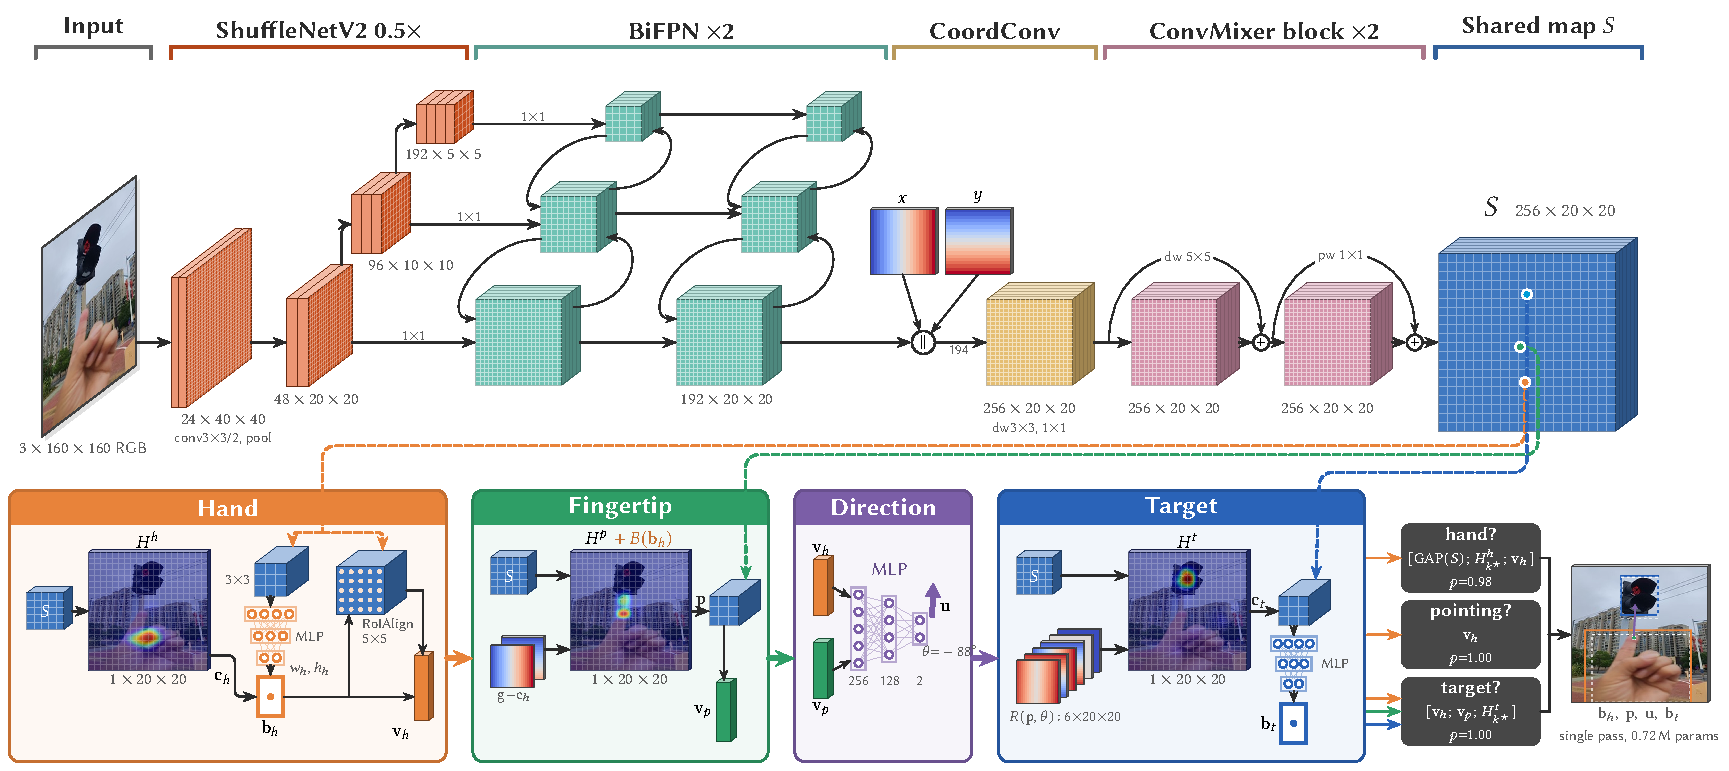
\includegraphics[width=\textwidth]{figures/architecture}
  \caption{SpatialNet. The trunk (top) turns one $160\times160$ frame into the shared map $S$ ($256\times20\times20$): ShuffleNetV2 stages at strides 8, 16 and 32, two BiFPN layers, CoordConv with reduction to 256 channels, and two ConvMixer blocks. Four heads (middle) run in order. Dashed lines mark where a head samples $S$ at the location the previous head predicted: the hand centre $\cH$, the fingertip $\tip$ and the target centre $\cT$. The direction head reads only the descriptors $\vH,\vP$. Right: the presence gates and the decoded output. Heatmaps, offset and ray-coordinate maps, gate probabilities and the output are real outputs of the trained model on one test image; each heatmap is overlaid on the input frame and scaled to its maximum.}
  \Description{Block diagram drawn as three-dimensional tensor slabs. The input frame passes through a ShuffleNetV2 backbone whose three scales feed two BiFPN layers by 1x1 projections; the 20x20 output gets two coordinate channels, is reduced to 256 channels and passes two ConvMixer blocks to give the shared map S. Four coloured panels show the heads in sequence: wearer hand (heatmap, 3x3 sample and MLP for the box size, RoIAlign descriptor), fingertip (heatmap from S and offset channels to the hand centre plus a hand-box prior, 3x3 sample giving the fingertip descriptor), pointing direction (an MLP on the hand and fingertip descriptors giving a unit vector), and pointed target (six ray-coordinate maps and S giving the target heatmap, 3x3 sample and MLP giving the box). Dashed lines from S show where each head samples it. On the right, three presence gates list their inputs and probabilities, and the output frame shows the predicted hand box, fingertip, direction and target box.}
  \label{fig:arch}
\end{figure}

\subsection{Shared Trunk}\label{sec:trunk}
The frame is resized to $160\times160$. A ShuffleNetV2~0.5$\times$ backbone~\cite{ma2018shufflenet} (stages 2--4 only; ImageNet-pretrained~\cite{deng2009imagenet}) gives feature maps at strides 8, 16 and 32. Two BiFPN layers~\cite{tan2020efficientdet} merge them into one $192\times20\times20$ map at stride 8. Each fused map is smoothed by a depthwise $3\times3$ convolution, SiLU, and parameter-free SimAM attention~\cite{yang2021simam}. We then append two coordinate channels (CoordConv~\cite{liu2018coordconv}) and reduce to $D{=}256$ channels with a depthwise-separable convolution. Two ConvMixer-style residual blocks~\cite{trockman2023patches} follow, each made of a depthwise $5\times5$ and a pointwise convolution with residual connections; their batch-norm scales start at zero, so each block is the identity at initialisation. The output is the shared map $S\in\mathbb{R}^{256\times20\times20}$, which all heads read. A $20\times20$ grid gives 8-pixel cells at the model input; the heads recover points with sub-cell precision (Section~\ref{sec:softargmax}), so a finer grid would mostly add compute. Sharing one map keeps the heads cheap: the largest head has 104K parameters (Table~\ref{tab:params}).

\subsection{Locating One Instance: Peak-Windowed Soft-Argmax}\label{sec:softargmax}
Each head predicts a $20\times20$ logit map $H$ and turns it into a point. A global soft-argmax~\cite{sun2018integral} returns the probability-weighted mean over all cells; when two hands are visible, that mean falls \emph{between} them. We therefore restrict the softmax to a $(2r{+}1)\times(2r{+}1)$ window $\mathcal{W}$ around the arg-max cell $k^\star$:
\begin{equation}
\pi_k=\frac{\mathbb{1}[k\in\mathcal{W}]\,\exp(\tau H_k)}{\sum_{j\in\mathcal{W}}\exp(\tau H_j)},\qquad
\hat{\vect{c}}=\sum_k \pi_k\,\cell_k ,
\label{eq:softargmax}
\end{equation}
where $\cell_k\in[0,1]^2$ is the normalised position of cell $k$ and $\tau$ is a temperature. The estimate follows a single peak, is differentiable within the window, and is not limited to cell centres. We use $(\tau,r)=(8,2)$ for the hand and the target and $(10,1)$ for the fingertip. The peak logit $H_{k^\star}$ is also passed to the gates as a confidence cue.

\subsection{Instance-Anchored Heads}\label{sec:heads}

\paragraph{Wearer's hand.} A depthwise $3\times3$ and pointwise head gives hand-centre logits $H^h$, and Eq.~\eqref{eq:softargmax} gives the centre $\cH$. For the box size $(w_h,h_h)$, we sample a $3\times3$ neighbourhood of $S$ around $\cH$ bilinearly (one-cell spacing). A depthwise $3\times3$ convolution and a pointwise projection collapse it to 128 dimensions, and a two-layer MLP with a sigmoid maps it to the size, giving $\bH=(\cH,w_h,h_h)$. To describe \emph{this} hand instance, we sample a $5\times5$ RoIAlign-style lattice~\cite{he2017mask} over $\bH$ enlarged by 1.15, collapse it to 128 dimensions, and fuse it with the box coordinates into the hand descriptor $\vH\in\mathbb{R}^{128}$.

\paragraph{Fingertip.} The fingertip must belong to the hand just found. Its logits add three terms:
\begin{equation}
H^p = V^p(S) + G^p\big([S;\,\alpha_p(\cell-\cH)]\big) + B(\bH).
\label{eq:tip}
\end{equation}
$V^p$ is a visual head of the same form as the hand head. $\alpha_p(\cell-\cH)$ are two channels holding each cell's offset to the hand centre, with a learnable scale $\alpha_p$, and $G^p$ is a small branch (a $1\times1$ convolution to 48 channels, then a $3\times3$ convolution to one channel, with its last layer initialised at zero) that learns where fingertips lie relative to the hand centre. $B$ is a fixed log-prior that is zero inside the hand box dilated by $\delta{=}1.3$ and falls linearly outside it:
\begin{equation}
B_k(\bH) = -\frac{\lambda}{\tau_p}\Big(\big[\tfrac{|g_{k,x}-c_{h,x}|}{\delta w_h/2}-1\big]_+ + \big[\tfrac{|g_{k,y}-c_{h,y}|}{\delta h_h/2}-1\big]_+\Big),
\end{equation}
where $[\cdot]_+=\max(\cdot,0)$. With $\lambda{=}4$, the penalty after the softmax temperature $\tau_p$ is 4 logits for every half box-width outside the dilated box, and no gradient flows from the prior into $\bH$. In the training labels, the fingertip lies inside the dilated box in 99.4\% of pointing images, so the prior rarely contradicts a label while it rules out the fingertips of other hands. Eq.~\eqref{eq:softargmax} (with $r{=}1$) gives the fingertip $\tip$, and a $3\times3$ sample around it gives the fingertip descriptor $\vP\in\mathbb{R}^{128}$.

\paragraph{Pointing direction.} An MLP ($256\to128\to2$, $\tanh$) maps $[\vH;\vP]$ to a vector, which we L2-normalise into the unit direction $\dir=(\cos\theta,\sin\theta)$ in image coordinates. The direction is supervised with the image-plane direction from the labelled fingertip to the labelled target centre (Section~\ref{sec:losses}), so $\dir$ is the direction \emph{to the target} as it appears in the image, not the 3D orientation of the finger.

\paragraph{Pointed target.} The target head is given the geometry of the predicted ray explicitly. From $\tip$ and $\dir$, every cell $k$ receives six \emph{ray coordinates} (inset in Figure~\ref{fig:arch}):
\begin{equation}
\Delta_k=\alpha_t(\cell_k-\tip),\qquad
t_k=\Delta_k\cdot\dir,\qquad
s_k=\big|\Delta_{k,x}\sin\theta-\Delta_{k,y}\cos\theta\big|,\qquad
\cos\theta,\qquad \sin\theta .
\label{eq:raycoords}
\end{equation}
These are the scaled offset from the fingertip (two channels), the signed distance along the ray (negative behind the fingertip), the distance from the line of the ray, and the direction itself. The target logits are
\begin{equation}
H^t = V^t(S) + G^t\big([S;\,R(\tip,\theta)]\big),
\label{eq:target}
\end{equation}
where $R$ stacks the six maps, and $G^t$ (13K parameters) has the form of $G^p$ and also starts at zero. The soft-argmax applies a softmax to $\tau H^t$, so $\pi_k\propto\exp(\tau V^t_k)\exp(\tau G^t_k)$: the geometry term acts as a learned \emph{multiplicative prior} on the visual evidence. Because $G^t$ starts at zero, training begins with a purely visual head, and the network uses the ray only as far as it lowers the loss. We let the network learn the shape of this prior, instead of fixing a cone, because the right shape depends on the gap: when the fingertip overlaps the target (about 70\% of EgoPoint targets, Section~\ref{sec:data}), the target centre can lie in any direction from the fingertip, while for large-gap targets a narrow band along the ray is informative. Whether the network exploits this freedom is an empirical question; Section~\ref{sec:ablations} shows that on EgoPoint it learns mainly a fingertip-proximity prior. The target centre $\cT$ follows from Eq.~\eqref{eq:softargmax}, and its size comes from a $3\times3$ sample, as for the hand, giving $\bT=(\cT,w_t,h_t)$.

\begin{table}[t]
  \caption{Parameters per module. FLOPs are counted by PyTorch's \texttt{FlopCounterMode} (one multiply--accumulate = 2 FLOPs; bilinear sampling not counted) for one $160\times160$ frame. Sizes are serialised state dictionaries.}
  \label{tab:params}
  \small
  \begin{tabular}{lrl}
    \toprule
    Module & Parameters & Role \\
    \midrule
    ShuffleNetV2 0.5$\times$, stages 2--4 & 143,136 & backbone, ImageNet-pretrained \\
    BiFPN $\times2$ & 81,426 & multi-scale fusion to stride 8 \\
    CoordConv + reduce & 52,310 & $194\to256$ channels \\
    ConvMixer $\times2$ & 145,920 & context mixing ($5\times5$ depthwise) \\
    \midrule
    Hand head & 104,259 & heatmap, size, descriptor $\vH$ \\
    Fingertip head & 51,826 & incl.\ 12,913 in the hand-offset branch $G^p$ \\
    Direction MLP & 33,154 & $[\vH;\vP]\to\dir$ \\
    Target head & 60,404 & incl.\ 13,105 in the ray branch $G^t$ \\
    Gates (hand / pointing / target) & 24,769 / 8,321 / 16,577 & presence logits \\
    Learnable scales $\alpha_p,\alpha_t$ & 2 & \\
    \midrule
    \textbf{Total} & \textbf{722,104} & 0.231 GFLOPs; 3.0\,MB FP32; 1.6\,MB FP16 \\
    \bottomrule
  \end{tabular}
\end{table}

\subsection{Presence Gates and Scene Decoding}\label{sec:gates}
Three MLP gates output logits for whether the wearer's hand is present (from $[\mathrm{GAP}(S);\,H^h_{k^\star};\,\vH]$), whether it is pointing (from $\vH$ alone) and whether something is pointed at (from $[\vH;\vP;H^t_{k^\star}]$). At inference they form a cascade with threshold 0.5: if the hand gate is off, the frame is \emph{no hand}; otherwise the pointing gate and then the target gate decide between \emph{hand, not pointing}, \emph{pointing, no target} and \emph{pointing at a target}. The pointing and target gates read instance descriptors rather than the whole image, so that another person's pointing hand elsewhere in the frame is not meant to switch them on by itself. The hand gate also sees the global pool, so that a frame containing only other people's hands can be classed as having \emph{no wearer's hand}. EgoPoint contains only the first and last of the four scenes (Section~\ref{sec:data}), so we evaluate the hand gate and make no claims about the pointing and target gates.

\subsection{Training Objective}\label{sec:losses}
The loss is a weighted sum of 13 terms (weights in Appendix~\ref{app:weights}), each computed only on images whose label contains the parts it needs. \emph{Localisation} uses the CIoU loss for the hand box~\cite{zheng2020distance}; the Wing loss~\cite{feng2018wing} for the fingertip, on normalised coordinates with $w{=}0.5$ and $\epsilon{=}0.1$; $1-\cos(\dir,\dir^\star)$ for the direction, where $\dir^\star$ is the unit vector from the labelled fingertip to the labelled target centre; and the SIoU loss~\cite{gevorgyan2022siou} plus $1-\mathrm{IoU}$ for the target box. \emph{Heatmaps} use the penalty-reduced focal loss of CornerNet and CenterNet~\cite{law2018cornernet,zhou2019objects} ($\alpha{=}2$, $\beta{=}4$) on Gaussian targets at the hand centre, fingertip and target centre ($\sigma$ = 1.5, 0.8 and 1.2 cells), which gives each heatmap a direct signal in addition to the gradient through the soft-argmax. \emph{Gates} use focal binary cross-entropy~\cite{lin2017focal} ($\gamma{=}2$), each on its own population (the hand gate on all images, the pointing gate on hand images, the target gate on pointing images), with positives weighted $2\times$ ($3\times$ for the hand gate), because a missed pointing gesture costs the user more than a false alarm that the interface can ignore.

\emph{Geometric consistency} adds two terms that use predictions only. The ray-alignment term asks the predicted target centre to lie on the predicted ray, in front of the fingertip:
\begin{equation}
\mathcal{L}_{\mathrm{ray}} = \big\|\vect{r}-(\vect{r}\cdot\hat{\dir})\,\hat{\dir}\big\| + 0.5\,\big[-\vect{r}\cdot\hat{\dir}\big]_+,\qquad \vect{r}=\hat{\vect{c}}_t-\hat{\tip}.
\end{equation}
Because $\dir^\star$ runs from the labelled fingertip to the labelled target centre, the ground truth gives $\mathcal{L}_{\mathrm{ray}}=0$ exactly: the term does not move the optimum and only penalises predictions that disagree with each other. For a fixed angular error, it grows with the fingertip--target distance, so it weighs large-gap targets most. The hand-axis term is a hinge that keeps $\hat{\dir}$ within $60^\circ$ of the axis from the predicted hand centre to the predicted fingertip. It is only a weak plausibility prior: the labelled direction lies inside this cone in 68.6\% of training images (64.1\% for overlap targets and 83.6\% for large-gap targets), so it has the smallest weight of all 13 terms. Ablation A2 (Section~\ref{sec:ablations}) removes both consistency terms.

\subsection{Learning Whose Hand It Is}\label{sec:ownership}
No public pointing dataset labels other people's hands, and EgoPoint frames contain only the wearer's. We therefore create distractors during training (Figure~\ref{fig:ownership}). The approach follows copy-paste augmentation~\cite{dwibedi2017cut,ghiasi2021simple}, but with the opposite aim: pasted hands are \emph{not} labelled, and the model is penalised for responding to them.

\begin{figure}[t]
  \centering
  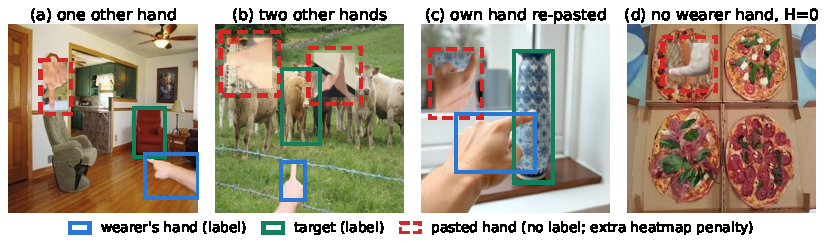
\includegraphics[width=\linewidth]{figures/ownership_examples}
  \caption{Distractor-hand pasting, produced by the training code. Pasted hands (red, dashed) come from other images (a, b) or from the same image (c), are rotated so that they rarely enter from the bottom edge, and are never labelled. A no-hand image with a pasted hand keeps the label \emph{no hand} (d).}
  \Description{Four training images. In the first two, one or two hands cut from other photos are pasted into the upper part of the image, rotated, and marked with red dashed boxes, while the wearer's pointing hand and the target keep their blue and green label boxes. In the third, a rotated copy of the wearer's own hand is pasted in the upper left. In the fourth, a pizza photo without a wearer's hand receives a pasted hand and keeps the label no hand.}
  \label{fig:ownership}
\end{figure}

With probability 0.5 for images with a hand and 0.3 for images without one, we paste one or two hand crops taken from other training images. The crops are rescaled, usually rotated (so that, unlike the wearer's arm, they rarely enter from the bottom edge), centred in the upper 65\% of the frame away from the wearer's hand and the target, and blended with a feathered mask; Appendix~\ref{app:aug} lists all settings. In 30\% of cases the pasted crop is the wearer's own hand from the same image, so that appearance alone cannot tell the two hands apart and the model has to use position, orientation and context. With probability 0.15, we also paste an unlabelled patch that contains no hand, so that a pasted rectangle is not itself a cue. Labels never change: in particular, a no-hand image with pasted hands remains \emph{no hand}, which teaches the hand gate to answer for the wearer only. In the hand-heatmap loss, the negative term near a pasted hand is multiplied by $1+4\,G_k$, where $G_k$ is a Gaussian ($\sigma{=}1.5$ cells) at that hand's centre, so that a response on another person's hand costs up to five times as much as one on background.

\emph{The prior this encodes.} The procedure assumes that, from a head-worn camera, the wearer's arm enters from the bottom of the frame, while other people's hands appear higher and in other orientations. This holds for most use of glasses but not always, for example when the wearer raises a hand above eye level or when a companion's hand is near the bottom of the view (Section~\ref{sec:discussion}).

\subsection{Scheduled Anchor Forcing}\label{sec:forcing}
Early in training, the predicted hand centre, fingertip and target centre are close to random, so the downstream heads would read features at meaningless locations. As in scheduled sampling for sequence models~\cite{bengio2015scheduled}, we sometimes replace each anchor with its ground-truth location, independently per image and per anchor, with a probability that decreases linearly from 0.5 to 0 over the first 20 epochs. From then on, training uses the model's own anchors, as at test time.
